\lecture{Herança}{inheritance}
\lecturetitle{\insertlecture}{\course}
\maketitle

\frame{
\Large
\frametitle{\insertlecture}
\begin{block}{Classes e objetos}
  \begin{itemize}
  \item Estrutura de uma classe;
  \item Atributos: tipos e literais;
  \item Modificadores;
  \item Construtor;
  \item Classes e objetos;
  \item Valor e referência.
  \end{itemize}
\end{block}
}

\if1=0
\begin{frame}[fragile]{Arranjos}

  \begin{definition}
    Arranjo é um contêiner de objetos que armazena um número fixo de
    valores do mesmo tipo. O comprimento do arranjo é estabelecido
    quando ele é criado. Depois da criação, seu tamanho é fixo.
  \end{definition}

  \begin{lstlisting}
    int[] arr; // declara um arranjo de inteiros
    arr = new int[8]; // aloca memoria para 8 inteiros
  \end{lstlisting}

Arranjo de objetos

\begin{lstlisting}
  CorpoCeleste[] viaLactea = new CorpoCelete[8]; 
\end{lstlisting}

  
\end{frame}

\large
\begin{frame}{Prática}
  \begin{enumerate}
  \item Fazer uma classe chamada {\tt Veiculo} com os seguintes
    atributos: {\tt marca}, {\tt modelo}, {\tt ano}, {\tt cor} e {\tt
      id} (identificador). O identificador é um atributo de classe e é
    incrementado a cada nova instância de um objeto {\tt Veiculo}.
    Nesta mesma classe, implemente um construtor para atribuir valores
    iniciais ao atributos, bem como os métodos {\it getters} e {\it
      setters}.
  \item Instancie 3 objetos fornecendo valores aos atributos através
    do construtor com parâmetros e respeitando o ocultamento dos
    atributos. Utilize um arranjo para agrupar os 3 objetos e imprimir
    os atributos em lote.
  \end{enumerate}
  
\end{frame}
\fi

\begin{frame}{Herança}
  
  \begin{block}{Herança simples}
    \small
    \begin{itemize}
    \item Em Java só é permitida herança simples de implementação e a
      múltipla é delegada somente para as interfaces, diferente de
      outras linguagens orientadas a objetos como C++ que permitem
      herança múltipla de implementação.
      \item A justificativa para esta decisão de projeto é a
        eliminação de possíveis ambiguidades que podem ser provocadas
        pela \alert{herança diamante}.
    \end{itemize}
    \end{block}


    \begin{block}{Herança diamante}
      \footnotesize
      \begin{columns}
        \begin{column}{.4\textwidth}
          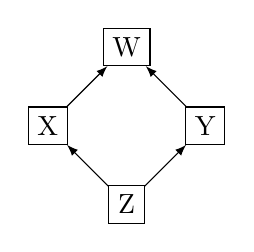
\begin{tikzpicture}[every node/.style={rectangle,draw},
            every path/.style={->,>=latex,draw}]
            \node (W) at (0,0) {W};
            \node (Y) at (1,-1) {Y};
            \node (X) at (-1,-1) {X};
            \node (Z) at (0,-2) {Z};
            \path (Z) -- (Y);
            \path (Z) -- (X);
            \path (Y) -- (W);
            \path (X) -- (W);
            
          \end{tikzpicture}
        \end{column}

        \begin{column}{.65\textwidth}
          Supondo que um objeto do tipo {\tt W} chamado {\tt wref}
          tenha uma variável chamada {\tt wVar}. Uma cópia de {\tt
            wVar} em um objeto do tipo {\tt Z} refere-se à cópia {\tt
            wVar} de {\tt X} ou de {\tt Y}, ou da cópia compartilhada
          proveniente de {\tt W}?
        \end{column}

      \end{columns}

  \end{block}

\end{frame}


% \begin{frame}[fragile]{Pré-requisito: Pacote}

%   \begin{definition}
%     Um pacote é um conjunto de classes agrupadas de acordo com algum
%     critério.
%   \end{definition}

%   \lstset{emph={package}, emphstyle={\bf \color{red}}}
%   \begin{lstlisting}
%     /* A classe deve estar no diretorio: */
%     /* Unix: $CLASSPATH/xyz/holanda/equipamento */
%     /* Windos: $CLASSPATH\org\adrianoholanda\equipamento */
    
%     package xyz.holanda.equipamento;

%     public class PlacaControladora {
%       ...
%     }
%   \end{lstlisting}

% \end{frame}


% \begin{frame}[fragile]{Carregamento}
% \small
%   \begin{block}{Caminho das classes}
%     As classes serão procuradas nos diretórios contidos na variável de
%     ambiente {\tt \$CLASSPATH} ou fornecidos à máquina virtual como
%     parâmetro usando a {\it flag} {\tt -classpath}.
%   \end{block}
  
%   Exemplo:
%   {\tt\scriptsize\noindent  \$ java -classpath=/home/holanda \\
%     \hspace{2cm}xyz.holanda.equipamento/Main}

%   \lstset{emph={import}, emphstyle={\bf \color{red}}}
%   \begin{lstlisting}
%     /* importa todas as classes do pacote */
%     import xyz.holanda.equipamento.*;
%     public class Main {
%       PlacaControladora pc;
%     }
%   \end{lstlisting}

%   \pause

%   \begin{lstlisting}
%     /* importa somente a classe especificada */
%     import xyz.holanda.equipamento.PlacaControladora;
%     public class Main {
%       PlacaControladora pc;
%     }
%   \end{lstlisting}
  
% \end{frame}


% \begin{frame}[fragile]{Modificador {\tt final}}
% \scriptsize
%   O modificador {\tt final} possui diferentes comportamentos para
%   diferentes contextos.

%   \begin{description}
%   \item[Atributo:] O atributo não pode ser modificado.
%   \item[Classe:] A classe não pode ser estendida.
%   \item[Método:] O método não pode ser sobreescrito ou sobrecarregado.
%   \end{description}
% \vspace{-0.33cm}
%   \pause
%   \lstset{emph={final}, emphstyle={\bf \color{red}}}
%   \begin{block}{\small Exemplos}
%     \begin{lstlisting}
%       /* Modo de declarar um atributo constante */
%       static final double PI = 3.14159265;
%       ...
%     \end{lstlisting}

%     \pause

%     \begin{lstlisting}
%       /* O conteudo da classe nao pode ser 
%       herdado por nenhuma outra classe */
%       final class Dinossauro {...}
%     \end{lstlisting}

%     \pause
    
%     \begin{lstlisting}
%       final boolean validaSenha(String usuario, String senha) {
%         boolean estaOK = false;
%         ...
%         return estaOK;
%       }
%     \end{lstlisting}
    
%   \end{block}

% \end{frame}


\begin{frame}[fragile]{Interface}
  \small
  \begin{itemize}
  \item As interfaces especificam os métodos a serem implementados
    pelas classes que se propõem a cumprir o contrato especificado
    pela interface. Em outras linguagens, como Objective-C, é chamado
    de \alert{Protocolo}.
  %\item Nas interfaces só são permitidas as declarações de atributos
   % constantes ({\tt static final}).
  \end{itemize}
    \begin{center}
      \begin{tikzpicture}[show background grid]\scriptsize
        \begin{interface}{Instrumento}{0,0}
          \operation{afinar()}
        \end{interface}

        \begin{class}{InstrumentoSopro}{3,-1.9}
          \implement{Instrumento}
          \operation{afinar()}
        \end{class}

        \begin{class}{Percursão}{0,-3.2}
          \implement{Instrumento}
          \operation{afinar()}
        \end{class}
        
        \begin{class}{InstrumentoCorda}{-3,-1.9}
          \implement{Instrumento}
          \operation{afinar()}
        \end{class}
        
      \end{tikzpicture}
  \end{center}
\end{frame}  

\begin{frame}[fragile]{Codificando}
  
  \begin{lstlisting}
    /* nome do arquivo: InstrumentoMusical.java */
    interface InstrumentoMusical {
      void tocar();
      void afinar();
    }
  \end{lstlisting}
  
  \begin{lstlisting}
    /* nome do arquivo: InstrumentoCorda.java */
    public class InstrumentoCorda implements InstrumentoMusical {
      void tocar() {
        System.out.println("Pressionar a corda!");
      }
      
      void afinar() {
        this.tocar();
        System.out.println("Esticar ou soltar a corda!");
      }
    }
  \end{lstlisting}
\end{frame}

\begin{frame}{{\tt protected}: este já é da família}
  O modificador \alert{{\tt protected}} força que o \alert{atributo}
  ou \alert{método} protegido só sejam utilizados pelas classes que
  herdarem a classe da qual faz parte.
  \hspace{-1.33cm}
    \begin{center}
      \begin{tikzpicture}
      \begin{abstractclass}{InstrumentoCorda}{0,0}
        \attribute{numCordas : int}

        \operation{\# afinar()}
      \end{abstractclass}
      
      \begin{class}{Guitarra}{0,-3}
        \inherit{InstrumentoCorda}
        \attribute{\# numCaptadores : int}

        \operation{\# afinar()}
      \end{class}
    \end{tikzpicture}
    
  \end{center}
  

\end{frame}


\begin{frame}[fragile]{Classe abstrata}
  \footnotesize
  As classes abstratas não podem ser instanciadas, mas possuem
  implementação e obrigatoriamente devem ser herdadas se houver a
  necessidade de utilização.
  
  \lstset{emph={abstract}, emphstyle={\bf \color{red}}}
  \begin{lstlisting}
    /* nome do arquivo: InstrumentoCorda.java */

    abstract class InstrumentoCorda implements InstrumentoMusical{
      protected int numeroCordas;
      
      void tocar() {
        System.out.println("Pressionar a corda!"); 
      }
      void afinar() {
        this.tocar();
        System.out.println("Esticar ou soltar a corda!"); 
      }
    }
  \end{lstlisting}
  
  \begin{lstlisting}
    /* nome do arquivo: Guitarra.java */
    public class Guitarra extends InstrumentoCorda {
      protected int numeroCaptadores;
    }
  \end{lstlisting}

\end{frame}

% \begin{frame}[fragile]{Exemplo classe abstrata}
%   \lstinputlisting[firstline=13]{code/src/org/adrianoholanda/poo/heranca/Teste.java}
% \end{frame}

\begin{frame}[fragile]{Composição x Herança}
  \small

  \begin{columns}
    \begin{column}{0.4\textwidth}
      \begin{block}{Composição}
         ``\alert{tem} um objeto do tipo''\\

        Exemplo:\\
        Um {\tt Carro} é composto por (tem) {\tt Roda}s, {\tt Motor}, {\tt
          Vidro}s, etc...
\begin{lstlisting}
class Carro{
  Roda[] rodas;
  Motor[] motor;
    ...
}
        \end{lstlisting}
        
      \end{block}

    \end{column}
    
    \begin{column}{0.4666\textwidth}
      
      \begin{block}{Herança}
        ``\alert{é} um objeto do tipo''\\

        Exemplo:\\
        Um {\tt Carro} é um {\tt Veiculo}.
        
\begin{lstlisting}
class Veiculo {...}
class Carro extends Veiculo {...}
\end{lstlisting}

      \end{block}

    \end{column}
  \end{columns}
  
\end{frame}


% \frame{\tableofcontents[currentsection]}
% \subsection{Polimorfismo}
% \frame{...}
% \section{}
% \frame{\tableofcontents[currentsection]}
% \subsection{}
% \frame{...}

